This document is a project report template for the School of Computer Science, University of Lincoln. It should give you some direction and instruction for formatting and presenting your project report. Currently, this template is designed for postgraduate project reports. However, the template can be modified fairly easily to conform to, for example, an undergraduate/MCOMP project report.

This document has been generated using \LaTeX, which is a widely used typesetting system in computer science, engineering, and other STEM disciplines. The following subsections of this chapter demonstrate some basic \LaTeX commands. If you would prefer to use the supplied LNCS Word template, then you should aim to replicate the formatting shown here.

\section{Formatting mathematics}
Here are two equations:

\begin{align}
a &= b + 1 \\
\frac{\hbar^2}{2m}\nabla^2\Psi + V(\mathbf{r})\Psi
&= -i\hbar \frac{\partial\Psi}{\partial t}    
\end{align}


And here is some text with some nice inline maths, $(x, y)$ wow $\gamma$ so cool $\rho$.

\section{Figures and Tables}

Here is a sentence, and you can see a nice picture in Figure \ref{fig:brayford}.

\begin{figure}[h]
    \centering
    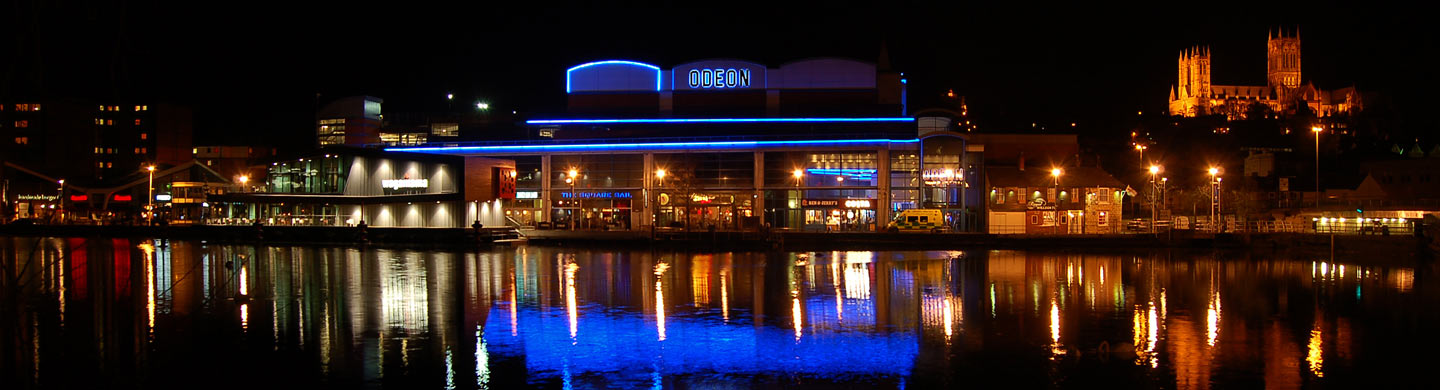
\includegraphics[width=\textwidth]{figures/brayford.jpg}
    \caption{A picture of the Brayford from Google Images.}
    \label{fig:brayford}
\end{figure}

Also, a table can be found in Table \ref{tbl:example-table}. You should use a \LaTeX~table generator like \url{https://www.tablesgenerator.com/} if you want to make your life easier.

\begin{table}[h]
    \caption{Here is a table. The caption goes above like this.}
    \centering
    \begin{tabular}{l|l|c}
        First name & Last name & Age \\
        \hline\hline
        Bob & Bobbington & 24 \\
        Benth & Wavies & 49 \\
        Joe & Bloggs & 37 \\
        Billy & Bob & 10 \\

    \end{tabular}
    \label{tbl:example-table}
\end{table}

\section{Referencing}
The included \texttt{[harvard]} in the document class command means that referencing will follow a Harvard style. You will be able to cite things inline with parentheses. You can do this by using \texttt{\textbackslash citep\{citekey\}}. It will print out something like this \citep{aad2012observation}. Or alternatively, you can use \texttt{\textbackslash cite\{citekey\}} to cite things like this \cite{chatrchyan2012observation}.

It is worth noting that the standard for referencing is Harvard, so you will not need to change this option. However, please double and triple check this to make sure you are using the correct referencing style. Also, ask your supervisor to make sure. This template uses Bib\LaTeX~for referencing, with a Biber backend. This is primarily due to the extensive features Bib\LaTeX~provides, along with the option of glossaries. If you want to customise the referencing style, you can either modify the template slightly to use different options, or use \texttt{\textbackslash usepackage} again to reimport it. There's probably some commands to change its options after its been imported too.

\subsection{Ludography}
This report template also contains an optional ludography. For Games Computing students to use this, just put references into your bib file as usual with the game's details. Then, make sure \texttt{keywords} is set to \texttt{\{game\}}. This is what is used to determine which references are games, and which are actual papers. For a more elaborate example, see \texttt{bib/ludography.bib}.

Also, make sure that the \texttt{title} key is actually the author of the game, and the \texttt{author} is the title of the game. The reason this is swapped around is because Bib\LaTeX~likes to print references out with the author first.

Then, just add \texttt{\textbackslash printLudography} with an optional title argument to print out all citations like \texttt{\textbackslash printLudography} or \texttt{\textbackslash printLudography[Games]}.

You can also use the \texttt{ludography} environment if you wish to print out some text before the list of games is printed. An example of this can be seen in \texttt{main.tex}.

To cite games, you can \texttt{\textbackslash cite} it like any other reference. However, if you want it to display the title instead of the standard referencing style, you can use \texttt{\textbackslash citeGame} instead.
